\chapter{Adaptive Learning Strategies}\label{approach}

This chapter explains our approach for adaptive neural paraphrase generation. It describes the main learning strategies that are used in detail including what purpose do they serve in our human-in-the-loop setting. First, details of the model which are used in the experiments are explained. Then descriptions of the datasets and the evaluation metric are presented. For last, the learning strategies and the experimental setups are discussed.

\section{Model Details}

In this work, a lightweight variant of the model proposed in  \cite{Prakashetal} with bahdanau attention \cite{bahdanau} is used. The reason the exact same model from the paper is not used is to fully explore all learning strategies since even with a lightweight version of the model, training takes a long time. The model keeps the same stacked LSTM based multi-layer architecture with residual connections but using 3 layers instead of 4. Figure 3 shows the basic unit in the model.

\begin{figure}[t]
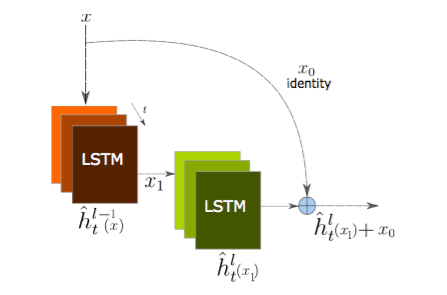
\includegraphics[width=\textwidth]{residualLSTM}
\centering
\caption{Stacked LSTM based model \cite{Prakashetal}.}
\end{figure}

During experiments, the model has 512 units in each LSTM layer with dropout probability of 0.3 after each layer. The model trains its own word embeddings with the embedding size of 512. For all experiments learning rate is started with 0.001 and decayed exponentially, with the square root function.

In the cases when it improves the performance, a beam search with beam size of 5 is used.

\section{Datasets and Evaluation Metric}

Four different datasets are used in the experiments varying in context and complexity. 

The Microsoft Research Paraphrase Corpuus (MSR) \cite{msrp} is a small but very challenging dataset which contains 5800 pairs of paraphrases extracted from news sources. Since the paraphrase pairs are extracted from different news sources the dataset contains a lot of lexical and contextual variety. It also contains a lot of special words and concepts. Because of these reasons MSR corpus is a very hard dataset to create paraphrases from even by the state-of-the-art model with high computational resources. The dataset is separated into subsets of 2753, 997 and 150 for training, test and validation respectively.

The Quora Question Pairs (QUORA) is a dataset consisting of question pairs which are labeled as paraphrases. It is originally a dataset for paraphrase recognition not paraphrase generation. The positive class of dataset is filtered and 155,000 paraphrase pairs are collected. There are one to many relationships in the dataset which means it contains multiple paraphrases for same source text. This property makes the dataset an ideal candidate for paraphrase generation. The dataset is separated into subsets of 119445, 22861 and 2000 for training, test and validation respectively.

The Microsoft Common Objects in Context (MSCOCO) \cite{mscoco} is a large dataset consisting of human generated image captions with 351,163 pairs. It also has one to many relationships. MSCOCO is one of the most popular datasets used in paraphrase generation literature. All of the dataset is used for training.

The PPDB Lexical (PPDB) \cite{ppdb} is a large dataset which contains 500,000 pairs of short paraphrases and it is also very popular in paraphrasing research. The paraphrases in this dataset are short that lack context information. All of the dataset is used for training.

\begin{table}
\small
 \begin{tabular}{||c c c c||} 
 \hline
 Label & Sentence & Dataset & \\ [0.5ex] 
 \hline
 source & the dvdcca then appealed to the state supreme court & MSR & \\
 \hline
 target & the dvd cca appealed that decision to the us supreme court & MSR & \\
  \hline
 source & why do rockets look white & QUORA & \\
 \hline
 target & why are rockets and boosters painted white & QUORA & \\
 \hline
 source & a blue and white bathroom with butterfly themed wall tiles & MSCOCO & \\
 \hline
 target & an angled view of a beautifully decorated bathroom & MSCOCO & \\
 \hline
 source & despicable & PPDB & \\
 \hline
 target & contemptible & PPDB & \\
 \hline
\end{tabular}
\caption{Example paraphrase pairs from the datasets.}
\end{table}


Table 3.1 shows example paraphrases from all the datasets used in the experiments. As it can be seen from the table, the datasets are varying in paraphrase complexity therefore it is easy to see why MSR dataset is harder to paraphrase than the others. MSR and QUORA datasets are used as target datasets on which the model is built and evaluated whereas MSCOCO and PPDB are used as source datasets for transfer learning.

There are no evaluation metrics especially designed for paraphrase generation. Therefore for evaluation the metric BLEU \cite{Papinenietal}  is used. BLEU is a widely used metric for paraphrase generation even though it is designed for machine translation. It is seen as a suitable option for paraphrase generation since it is shown that the score correlates well with human evaluation.

\section{Experimental Setups}

The human-in-the-loop data acquisition process is simulated by randomly dividing a dataset into train, test and validation, taking training set's subsets and feeding it to the model in each iteration. After each iteration the model is trained with the data available according to learning strategy which is experimented on and evaluate its performance iteratively with the test set. The test set is preferred to be relatively large in order to test how well the model generalize after each iteration. The model is trained with same amount of epochs and start the training with same hyperparameter configurations through the iterations in order to compare the performance without bias. If it is necessary, parameter tuning is done on validation set beforehand and the best model is taken for the experiments with learning strategies. Every learning strategy is experimented with the same model (same architecture, same hyperparameters etc.).

\section{Incremental Learning Strategies}

In the continuous setting this thesis studies, the training data is limited at the beginning. After a certain amount of time, the system is able to collect enough data to build a stable model with supervised learning. This model then, can be used for application purposes as long as it performs at an acceptable level. There are two major drawbacks in this solution. Firstly, the model is not able to use the training data which is collected after its creation. This is clearly a waste of resources since the training data comes from a continuous stream. Secondly and most importantly, the model would have to be trained on a regular basis just to keep up with the new training data. This is not desirable and not practical even impossible depending on the circumstances. Therefore, incremental learning is a natural option in this case.

The main concern in human-in-the-loop setting is to make continual, data-driven learning possible since traditional supervised learning is not practical. The model should keep learning with incoming training data which is provided by the data stream, adapt itself to the changes in dataset without forgetting the knowledge it learned before. Since the model is getting training data in small chunks, one of the most important design decisions which has to made is how to process available training data through time. In case of neural models learning basically means to update model's weights by iterations according to the training data. Because of the very nature of gradient descent based learning the more certain data points are used in training the more the model is going to adjust itself towards to those data points. This could lead to a bias towards the training data which is gathered at past, severely hurting the model's learning capability. It is important to notice that this can also happen within the same dataset if the dataset has high variance. This problem would not occur if the model is trained with supervised learning since the whole dataset would be available for training.

As explained in previous sections, concept drift is the other big challenge that has to be considered when learning in continuous data streams. Optimally model should be able to pick up the statistical and conceptual changes in the incoming training data and update its weights accordingly. The model should be able to do this without forgetting previously learned knowledge so that it can preserve its original functionality. After adapting to the new training data, it should still be able to perform reasonably well when it encounters test data from the original dataset. 

It is reasonable to say that when the two problems described above are considered, adaptivity of a model is basically a tradeoff between how fast it learns the new knowledge and how fast it forgets the old one. Any learning strategy that is to be used in adaptive learning, should employ some measures in order to preserve the balance between learning and forgetting. As it is said before because of the very nature of how deep neural models learn, it is impossible to avoid either one of them but it is possible control the rate of how fast the model learns and forgets.

Two different incremental learning strategies which differ in how they process the incoming training data, are proposed and experimented with. The model is regulated with different methods available in traditional supervised learning. The behaviour of these two incremental learning approaches are studied and some insights on adaptive paraphrase generation, are provided. The training and regularization methods that are used, are fairly simple but they haven't been studied before so the finding of this thesis is thought as a foundation for more complex approaches for adaptive learning in NLP.

\subsection{Incremental Learning with Data Pooling (IL1)}

The first learning strategy trains continuously (weights are not re-initialized between iterations, model uses and updates the same weights) from a data pool which contains all the data collected in previous iterations. The model uses all the data available to it regardless how old or new the data is. Figure 3.2 shows the basic work flow of the learning strategy. As it can be seen from the figure at the end of each iteration, the collected data is placed in a data pool and the model trains itself using the updated data pool. After the training process next iteration starts and cycle continues. The purpose of this learning strategy is mainly show that if the neural model can constantly improve itself through time to the incoming data. Main focus is not to forget previously attained knowledge while learning new training data reasonably well and make model to use all the resources available. The advantages of this learning strategy can be listed as:

\begin{figure}[t]
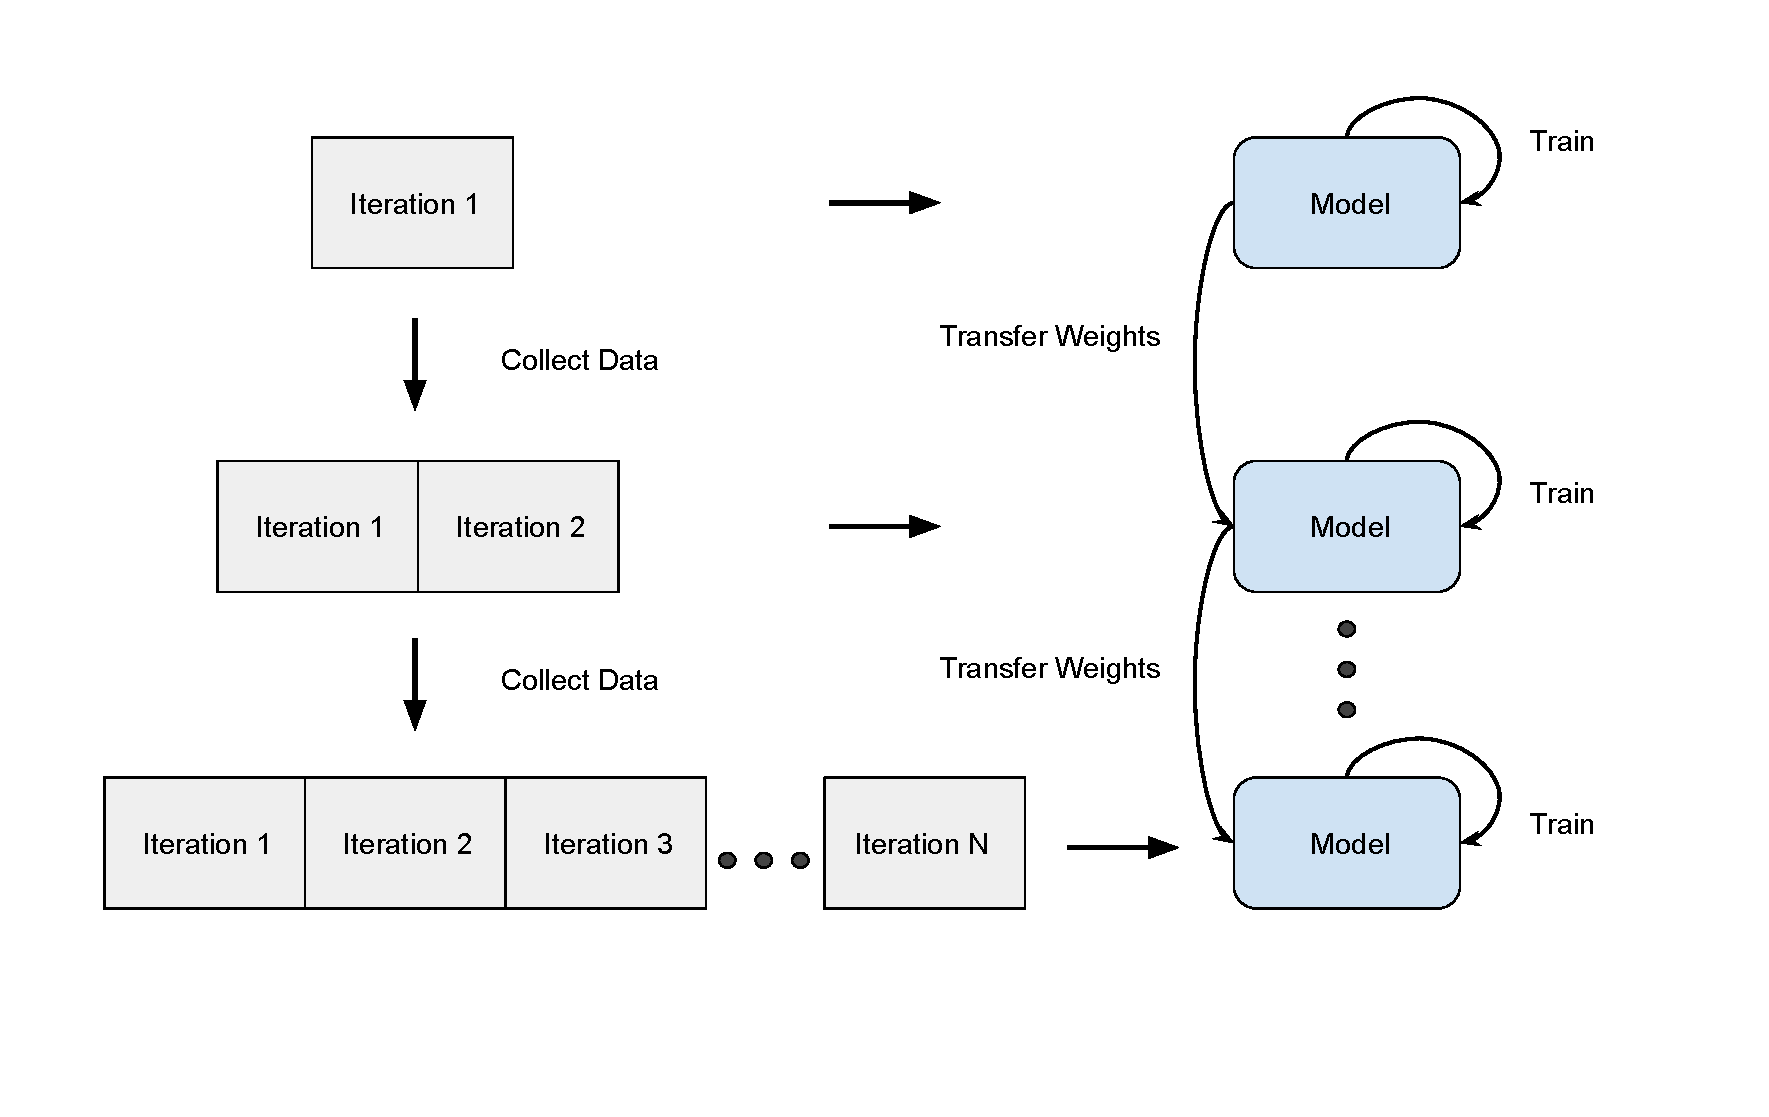
\includegraphics[width=\textwidth]{IL1}
\centering
\caption{Incremental learning with data pooling (IL1). The model uses data from all prevous iterations, hyperparameters re-initialized and weights are transferred through iterations.}
\end{figure}

\begin{itemize}

  \item Since the model trains on all data available at the end of each iteration, it is unlikely to forget learned knowledge from previous iterations.
  \item The model has the chance to learn more difficult data points better especially if they are encountered in early iterations. Basically instead of waiting to get enough data to learn with supervised learning, that time can be used to work on challenging data points seen by the model.

\end{itemize}

The disadvantages of this learning strategy are:

\begin{itemize}

  \item Since the size of data pool is increasing linearly, the time model takes to the end of each iteration and the required memory for data pool, increases as well. This increase can be linear or exponential depending on the model.
  \item The model sees data points from earlier iterations way more often which means it updates its weights according to those data points more often. This can cause overfitting to those particular data points which can diminish the performance of the model.

\end{itemize}

\subsection{Incremental Learning without Data Pooling (IL2)}

The second learning strategy trains continuously (weights are not re-initialized between iterations, model uses and updates the same weights) only from the data of last iteration. There is no data pool that aggregates collected training data. Figure 3.3 shows the basic work flow of the learning strategy. As it can be seen from the figure, the model only updates itself with the most recent iteration. After the training process next iteration starts and cycle continues. Purpose of this learning strategy is to create an efficient model in terms of the training time and memory. The main focus is the adaptivity of model to new data. The advantages of this learning strategy can be listed as:

\begin{figure}[t]
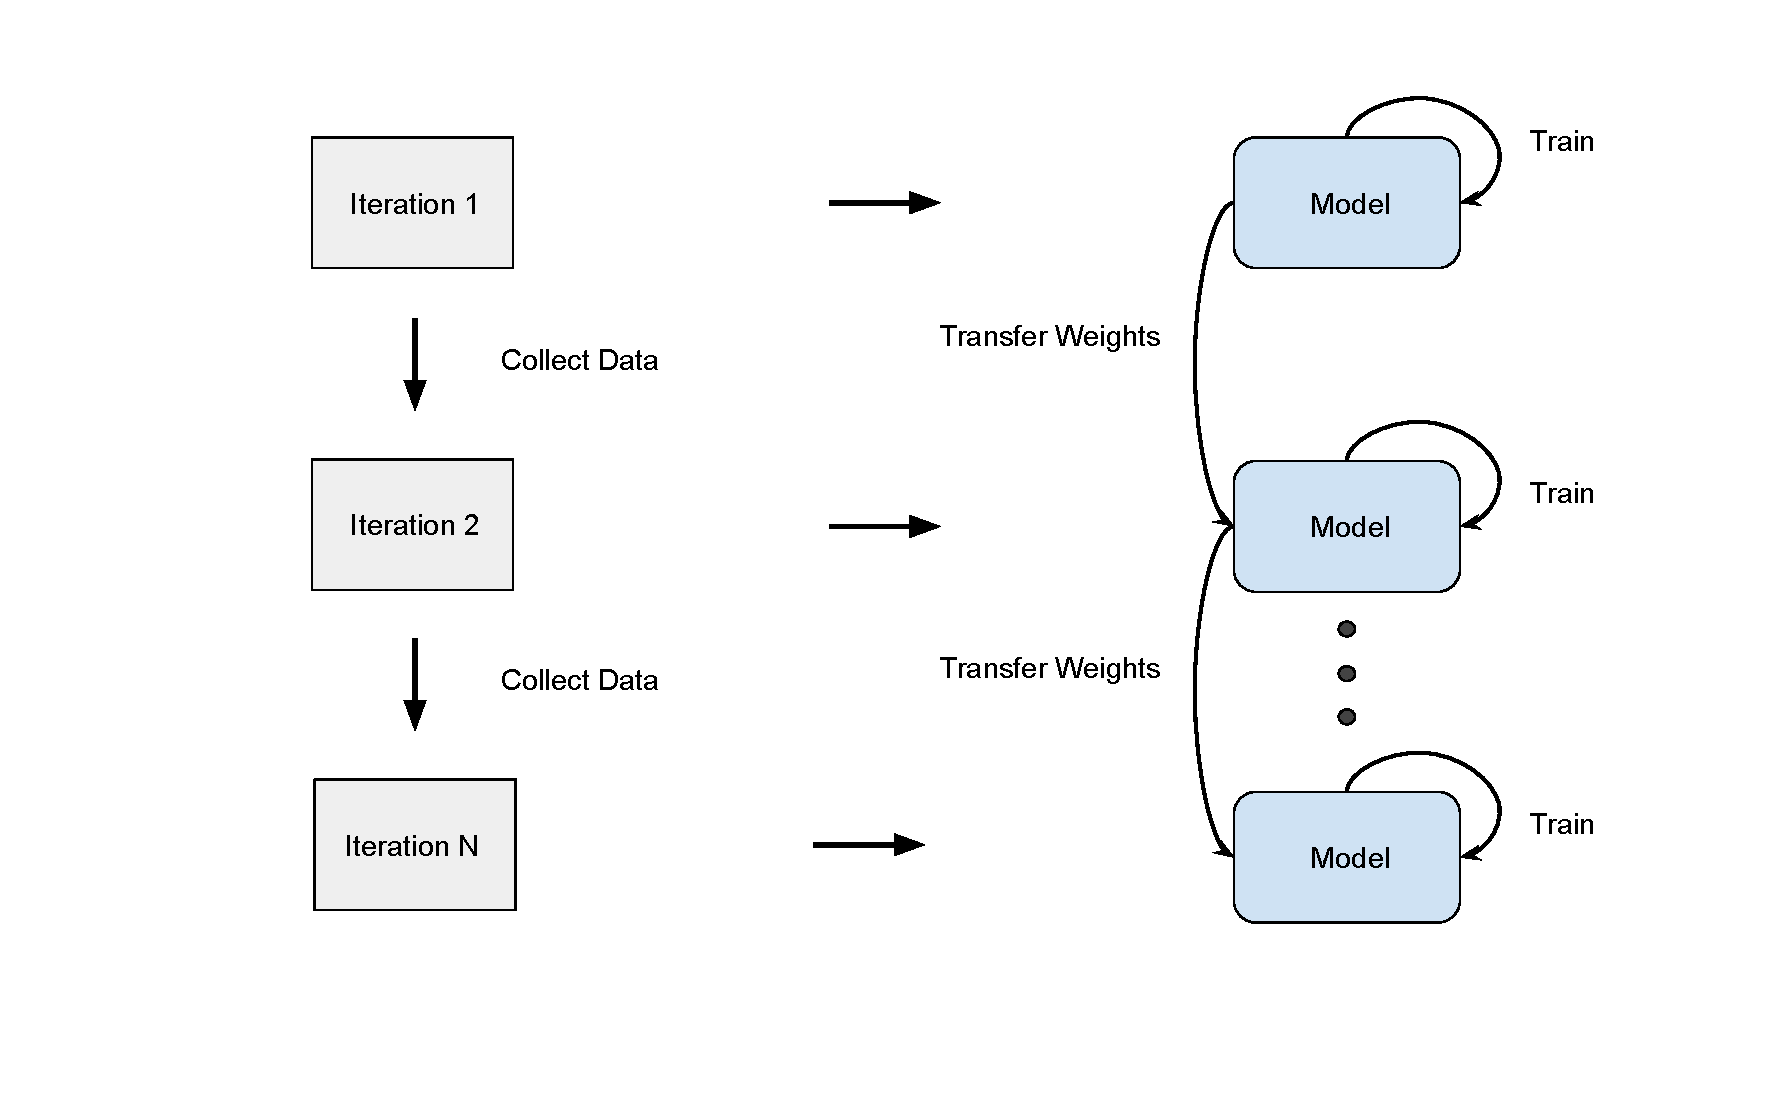
\includegraphics[width=\textwidth]{IL2}
\centering
\caption{Incremental learning without data pooling (IL2). The model only uses data from latest iteration, hyperparameters re-initialized and weights are transferred through iterations.}
\end{figure}


\begin{itemize}

\item Since the size of data pool is constant, it is efficient in terms of time and memory.
\item The model sees all data points for equal amount of times therefore it does not have the problem of overfitting as incremental learning with data pooling.

\end{itemize}


The disadvantages of this learning strategy are:

\begin{itemize}

\item Since the model trains on iterations separately it is prone to overwrite and forget old knowledge from previous iterations.
\item All training points are updated for same amount of iterations. If the number of epochs are not large enough the model can underfit and fail to generalize.

\end{itemize}

\subsection{Incremental Learning with Network Expansion (IL-NE)}

The last learning strategy trains continuously (weights are not re-initialized between iterations, model uses and updates the same weights) and expands the neural network after certain number of iterations. In this context network expansion means adding another LSTM layer to the network. Purpose of this learning strategy is to increase adaptive capabilities of the model. Main focus is to deal with possible concept drift which can occur during data acquisition. By adding randomly initialized new layers when more than a certain amount of data is introduced to the model, specialized layers focusing on old and new information are aimed to be created. Experiments are conducted with expansion in every third iteration and expansion only in the fifth iteration. Additionally, an experiment is done with freezing first active layer in every expansion step, studying if restricting the model through time helps with adaptivity.   

\subsection{Incremental Learning Baseline (IL3)}

The model is also trained from ground zero (with the weights re-initialized) from data pool at the end of every iteration in order to create a comparable baseline. The baseline model which is trained after the last iteration is basically the model trained with supervised learning since it uses the whole training data available. The basic idea is to check if the incremental learning strategies achieve better or comparable performances than last baseline model. Figure 3.4 shows how the baseline is created.

\begin{figure}[t]
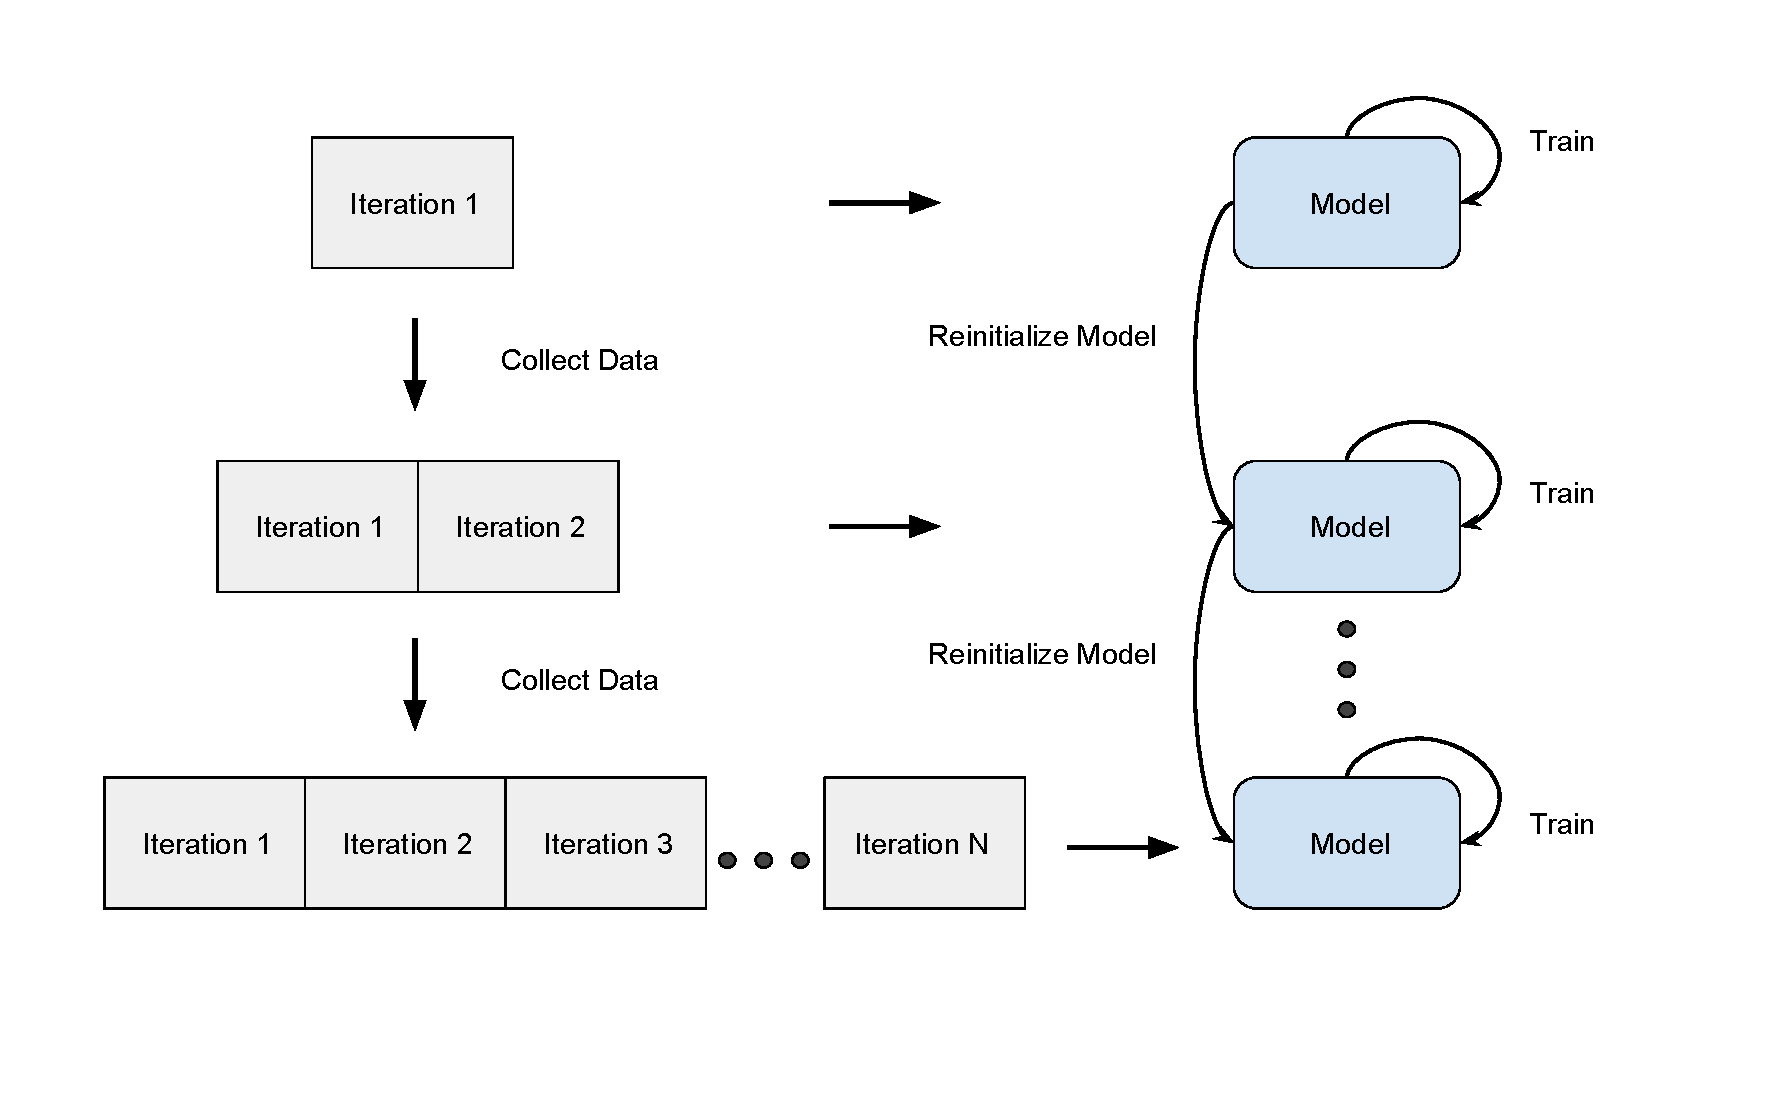
\includegraphics[width=\textwidth]{IL3}
\centering
\caption{Incremental learning baseline (IL3). The model is trained from scratch for each iteration, no knowledge transfer involved.}
\end{figure}

\subsection{Model Regularization in Incremental Learning}

Simple and well known regularization techniques are used with incremental learning strategies in order to control the tradeoff between old and new information. The regularization techniques that are used in the models are dropout, learning rate decay and layer freezing. Learning rate and its decay is used to control how large the weight updates are during the learning. A non-shared regularization mechanism is employed where every iteration has its hyperparameters re-initialized in order to make the model adaptive to most recent data. In other words while the weights of the network is transferred through iterations, the decayed learning rates are not.

In this case the assumption is a very small learning rate with high decay rate will make the model unresponsive to the latest iterations. Exponential learning rate decay (square root decay) is used in our experiments which means the learning rate will decrease through iterations. Dropout is used to prevent overfitting especially in incremental learning with data pooling where the model is updated for certain data points way more than the rest of dataset. Also a certain number of the layers are freezed so that corresponding layers' weights are not updated during training. The idea is to make sure that some of the previously learned knowledge is not overwritten by the incoming dataset. 

\section{Transfer Learning Strategies}

During incremental learning, the model is trained at the end of each iteration with training data specified by the chosen incremental learning strategy. Since the model is trained continuously without reinitializing the weights in each iteration, this is equivalent to transfer learning between iterations. In the initial experimental setups, the training data comes from the same dataset divided into subsets provided as iterations. This experiment setup is expanded by transferring knowledge from a different paraphrasing dataset and start the incremental learning process with a pre-trained model or in other words with a knowledge base. 

Transfer learning from other sources are extremely relevant to the continuous human-in-the-loop setting especially in the cases where there are no resources to collect a large dataset. Since the training data is collected iteratively the model would have to work with even smaller dataset at the beginning. Transfer learning can help the model to learn better, providing a better initialization in the worst case scenario and increase the performance in this case. 

More importantly by training a model in a different dataset and using the pre-trained model to learn a new dataset, an artificial equivalent of concept drift is simulated no matter what transfer strategy is used. Basically in this case, there is a model which is used for a different dataset (different statistics, distribution, context etc.) than the one it is trained with. Only difference between this scenario and the concept drift scenario that exists in incremental learning is, in this case the model has access to all of the new dataset, instead of small chunks. Therefore finding good strategies for transfer learning can help with the concept drift problem if the transfer strategies is combined with incremental learning. 

Before starting with the transfer learning from other paraphrase datasets, experiments are conducted for answering these questions:

\begin{itemize}

\item Is knowledge transfer possible for neural paraphrase generation?

In order to answer this question, a model is trained with a large paraphrasing dataset as a source model. Then the transfer is done from this source model to target model with simplest way possible which is copying the weights of every component of source model and train the target model in a supervised manner. The performance is compared with traditional supervised learning without transfer to see if there is any improvement.

\item If answer to the first question is yes, what components of the model are being transferred?

To see what aspects of the source model is transferred, the experiments are run with three different settings; transfer embedding layer only, transfer embedding and hidden layers, transfer all layers including output layers. The performances are compared to see what components lead to improvement. 

\item Does transfer success depend on the characteristics of the participant datasets?

In order to speculate about what properties of the datasets relevant to knowledge transfer, experiments with three different source datasets and two target datasets, are run. The transfer performances are studied to establish some correlations between performance and properties like context, content, size of the datasets.

\end{itemize}

After establishing knowledge transfer is indeed possible, three different transfer strategies are proposed:

\begin{itemize}

\item INIT: Knowledge transfer is done by copying every component of source model to target model.  

\item Freeze n-layers: Same as INIT but first n layers of the model are freezed.

\item Surplus layer:  Same as INIT but a surplus layer is added before output layer and all the other layers are freezed.

\end{itemize}

Basically, proposed transfer strategies are designed for putting restrictions on the target model, directly effecting how much the model learns from training data. Whereas INIT puts no restrictions on the target model, surplus layer conservatively keeps the knowledge from source model and freeze n-layers approach is thought as a middle ground between them, making adjustments between knowledge learned from source dataset and target dataset . With transfer learning the model deals with a similar old vs. new knowledge tradeoff as incremental learning but with a different scale. In this case old knowledge part of the tradeoff is much larger and can have significant effects on the models performance. Moreover all of the transfer strategies proposed in this chapter are designed while specific use cases are considered. It is hypothesized that INIT is more suitable when the dataset for target model is large and the model has to be complex whereas surplus layer is more suitable when the dataset for target model is small and the model has to specialize (general to specific for the same domain). 

The same regularization techniques used for incremental learning strategies are used for transfer learning strategies as well, even though their effect on the performance can be not the same. Since it is essential to efficiently use the knowledge learned from the source dataset in the target dataset, learning rate for the target model becomes very important. A large learning rate might overwrite the existing weights very quickly which means losing the information gained before. Therefore in the experiments, a larger learning rate is used for source dataset and smaller learning rate is used for target dataset. The same exponential learning decay that is used in incremental learning, is kept.

\section{Active Learning Strategies}

Active learning is perfectly suitable for human-in-the-loop setting since it aims to enable learning with less amount of data. Not only it can reduce the cost of data acquisition, it can also enhance the overall process since it enables the model to learn faster which would mean earlier and more meaningful involvement with the users. As it is explained before the core idea behind active learning is determining the most difficult data points to paraphrase and make the users annotate those data points. The aim is to integrate active learning into the incremental learning with data pooling strategy and study its effects on the model's performance. It is hypothesized that since incremental learning with data pooling updates its weights towards to some data points in the dataset more than others, if those points are made sure to be most difficult data points to paraphrase, this can help the model to train better and faster.

It is hard to define a difficult or informative data point in case of paraphrase generation just because of the fact that it is a generation task not classification or regression. Contrary to other NLP tasks like paraphrase recognition or named entity recognition, in paraphrase generation the model only has the source texts to work with which limits the information it has on the dataset. For example in the case of paraphrase recognition, the dataset contains both of the paraphrase pairs and the annotator is only have to decide if they have the same meaning or not but nevertheless information from both of the sentences can be used for sampling. In this case, the sampling strategies which consist of heuristics regarding the training data, are based on only the source texts. Three different sampling strategies are combined with incremental learning with data pooling. Sampling techniques that are used for the experiments are:

\begin{itemize}

\item Random Sampling (RS): Sentences which are going to be paraphrased by the user are selected randomly. This is the default method for all of the other experiments in this thesis and used as a baseline.

\item N-gram Coverage (NC): Proposed in \cite{rubio} for interactive machine translation, this sampling technique focuses on selecting the rarest data points in terms of their n-grams. In other words, this technique aims to calculate how much new information a data point can provide. The hypothesis is rarest sentences have to be seen more for model to learn an accurate probability estimation. 

Before the training, number of each n-gram present in the training data is calculated and stored. Since human-in-the-loop approach is simulated, n-gram counts of the whole dataset can be calculated beforehand but in a real world application where new training data is constantly streamed, they should be updated after each iteration. An n-gram is labelled as rare when it appears less than A times in training data. Using this label, the score for a given source sentence f, is computed as:

\begin{equation}
C(f) = \frac{\sum_{n=1}^N \lvert{\nu^{<A}_{n}(f)} \lvert} {\sum_{n=1}^N \lvert{\nu_{n}(f)} \lvert} 
\end{equation}


where ${\nu_{n}(f)}$ is the set of n-grams with size n in f, ${\nu^{<A}_{n}}$ is the set of n-grams of size n in f that are rare and N is the maximum n-gram order. In experiments with incremental learning with data pooling, N = 4 is chosen as the maximum n-gram order and a value of 10 is chosen for the threshold A. In order to asses how well n-gram coverage represents the informativeness of data, an experiment is conducted with reverse n-gram sampling where the data points are chosen based on how frequent they are in the dataset in terms of n-grams. The score for reverse n-gram sampling is calculated as:

\begin{equation}
C(f) = \frac{\sum_{n=1}^N \lvert{\nu^{>=A}_{n}(f)} \lvert} {\sum_{n=1}^N \lvert{\nu_{n}(f)} \lvert} 
\end{equation}

where the terms are the same as n-gram sampling equation.

%\item Least Confidence (LC): A very intuitive sampling technique, it chooses data points in which the model has least confidence in. In the context of deep neural models this means to select the data points that are assigned with lowest probability according to the equation \cite{shen}:
%
%\begin{equation}
%1 - \max_{y_{1}.....y_{n}}  \mathbb{P}  \left[ {y_{1}.....y_{n}}  | \{ x_{ij} \}  \right]   
%\end{equation}
%
%For LSTM based sequence-to-sequence model used in this work, the score for a data point is calculated by using the probability of greedily decoded sequence.

\end{itemize}

Since MSR dataset contains a very small number of paraphrases, active learning strategies are only tried on QUORA dataset.


